The wheeled-leg exploration rover SherpaTT is shown in \refFig{fig:sherpatt}. It is one of the subsystems comprising a \ac{MRS} developed at the \ac{DFKI}'s \ac{RIC}. The rover has undergone several field trial campaigns, particularly with a Mars analogue terrain field deployment  in Utah, USA, where a logistics chain for sample return was evaluated. The rover's versatility has been demonstrated through a multitude of tasks such as assembling surface deployable payloads, deploying BaseCamps, or using its \ac{RA} for soil sampling with modular \ac{PLI} sampling devices \citeother{Cordes2018}.

\begin{figure}[h]
  \centering
  \hypersetup{linkcolor=captionTextColor}
  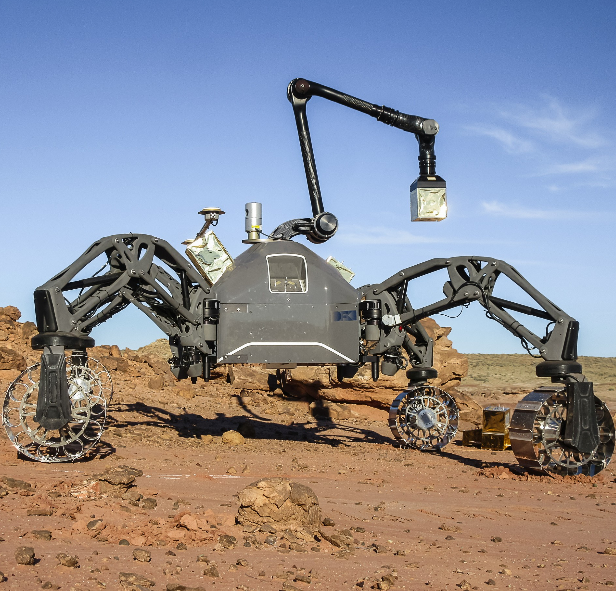
\includegraphics[width=0.5\linewidth]{sections/introduction/background/images/sherpa-tt.png}\\
  \caption[Exploration rover SherpaTT]
          {Exploration rover SherpaTT. Taken from \citeother{Cordes2018}.}
  \label{fig:sherpatt}
\end{figure}


SherpaTT's actively articulated suspension system consists of four wheeled-legs with a total of 20 motors. The distribution of motors across a single leg is shown in \refFig{fig:sherpatt-actively-articulated-suspension-system}. Each leg is equipped with three suspension motors and two drive motors. The suspension motors are responsible for Pan, \ac{IL}, and \ac{OL} revolute joint rotations whereas the drive motors are responsible for \ac{WS} and \ac{WD}.

\begin{figure}[h]
  \centering
  \hypersetup{linkcolor=captionTextColor}
  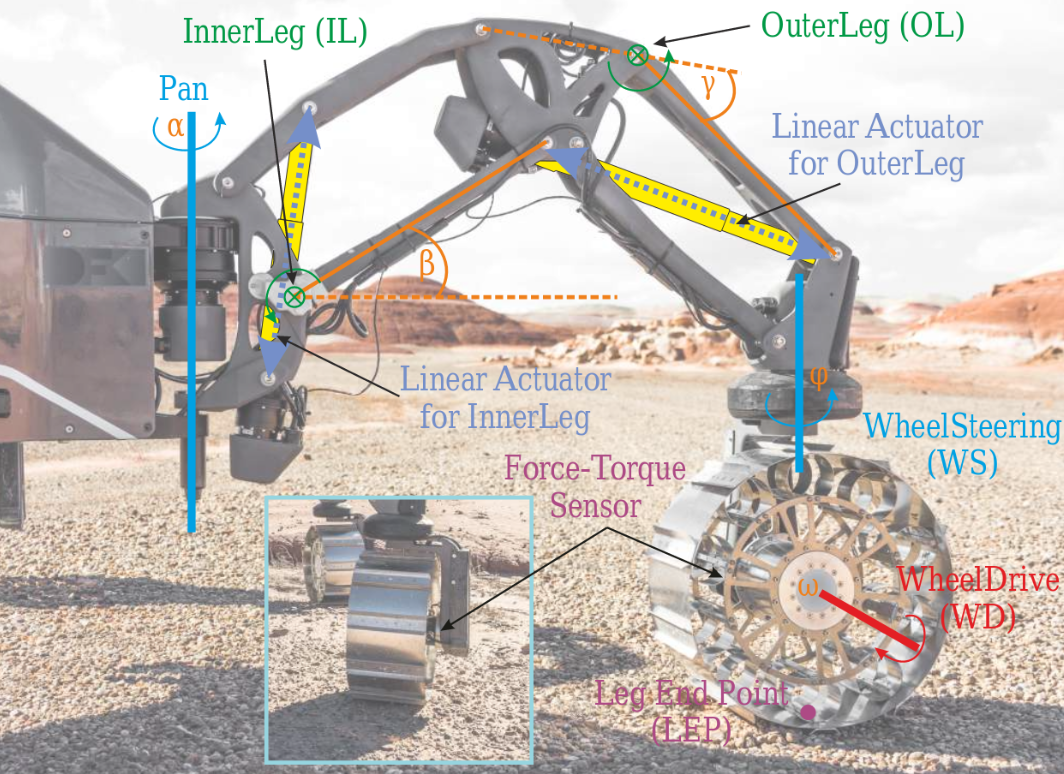
\includegraphics[width=0.6\linewidth]{sections/introduction/background/images/sherpatt-actively-articulated-suspension-sytem.png}\\
  \caption[SherpaTT actively articulated suspension system]
          {SherpaTT actively articulated suspension system. Taken from \citeother{Cordes2018}.}
  \label{fig:sherpatt-actively-articulated-suspension-system}
\end{figure}
